\documentclass[aspectratio=169]{beamer}\usepackage[]{graphicx}\usepackage[]{xcolor}
% maxwidth is the original width if it is less than linewidth
% otherwise use linewidth (to make sure the graphics do not exceed the margin)
\makeatletter
\def\maxwidth{ %
  \ifdim\Gin@nat@width>\linewidth
    \linewidth
  \else
    \Gin@nat@width
  \fi
}
\makeatother

\definecolor{fgcolor}{rgb}{0.345, 0.345, 0.345}
\newcommand{\hlnum}[1]{\textcolor[rgb]{0.686,0.059,0.569}{#1}}%
\newcommand{\hlsng}[1]{\textcolor[rgb]{0.192,0.494,0.8}{#1}}%
\newcommand{\hlcom}[1]{\textcolor[rgb]{0.678,0.584,0.686}{\textit{#1}}}%
\newcommand{\hlopt}[1]{\textcolor[rgb]{0,0,0}{#1}}%
\newcommand{\hldef}[1]{\textcolor[rgb]{0.345,0.345,0.345}{#1}}%
\newcommand{\hlkwa}[1]{\textcolor[rgb]{0.161,0.373,0.58}{\textbf{#1}}}%
\newcommand{\hlkwb}[1]{\textcolor[rgb]{0.69,0.353,0.396}{#1}}%
\newcommand{\hlkwc}[1]{\textcolor[rgb]{0.333,0.667,0.333}{#1}}%
\newcommand{\hlkwd}[1]{\textcolor[rgb]{0.737,0.353,0.396}{\textbf{#1}}}%
\let\hlipl\hlkwb

\usepackage{framed}
\makeatletter
\newenvironment{kframe}{%
 \def\at@end@of@kframe{}%
 \ifinner\ifhmode%
  \def\at@end@of@kframe{\end{minipage}}%
  \begin{minipage}{\columnwidth}%
 \fi\fi%
 \def\FrameCommand##1{\hskip\@totalleftmargin \hskip-\fboxsep
 \colorbox{shadecolor}{##1}\hskip-\fboxsep
     % There is no \\@totalrightmargin, so:
     \hskip-\linewidth \hskip-\@totalleftmargin \hskip\columnwidth}%
 \MakeFramed {\advance\hsize-\width
   \@totalleftmargin\z@ \linewidth\hsize
   \@setminipage}}%
 {\par\unskip\endMakeFramed%
 \at@end@of@kframe}
\makeatother

\definecolor{shadecolor}{rgb}{.97, .97, .97}
\definecolor{messagecolor}{rgb}{0, 0, 0}
\definecolor{warningcolor}{rgb}{1, 0, 1}
\definecolor{errorcolor}{rgb}{1, 0, 0}
\newenvironment{knitrout}{}{} % an empty environment to be redefined in TeX

\usepackage{alltt}

% Set lecture number for later use


% Part common to all the lectures
\subtitle{MATH 2740 -- Mathematics of Data Science -- Lecture 05}
\author{\texorpdfstring{Julien Arino\newline\url{julien.arino@umanitoba.ca}}{Julien Arino}}
\institute{Department of Mathematics @ University of Manitoba}
\date{Fall 202X}

% Title of the lecture
\title{Matrix methods -- Least squares problems}



\usetheme{default}
% Slide setup, colour independent

\usepackage{amsmath,amssymb,amsthm}
\usepackage[utf8]{inputenc}
\usepackage{colortbl}
\usepackage{bm}
\usepackage{xcolor}
\usepackage{dsfont}
\usepackage{setspace}
% To use \ding{234} and the like
\usepackage{pifont}
% To cross reference between slide files
\usepackage{zref-xr,zref-user}
% Use something like
% \zexternaldocument{fileI}
% in the tex files. And cite using \zref instead of \ref

% Cross-reference system - see CROSS-REFERENCE-SETUP.md for manual setup instructions
\usepackage{booktabs}
\usepackage{marvosym}
\usepackage{cancel}
%\usepackage{transparent}
% Make doi clickable in the bibliography?
\usepackage{doi}

\usepackage[T1]{fontenc}

\usepackage{longtable}

% For heavier titles
\usepackage{helvet} % Enables Helvetica font family


% Fields and the like
\def\IC{\mathbb{C}}
\def\IE{\mathbb{E}}
\def\IF{\mathbb{F}}
\def\II{\mathbb{I}}
\def\IJ{\mathbb{J}}
\def\IK{\mathbb{K}}
\def\IM{\mathbb{M}}
\def\IN{\mathbb{N}}
\def\IP{\mathbb{P}}
\def\IR{\mathbb{R}}
\newcommand{\IRplus}{\mathbb{R}_{\ge 0}}
\def\IZ{\mathbb{Z}}
\def\11{\mathds{1}}


% Bold lowercase
\def\ba{\bm{a}}
\def\bb{\bm{b}}
\def\bc{\bm{c}}
\def\bd{\bm{d}}
\def\be{\bm{e}}
\def\bf{\bm{f}}
\def\bg{\bm{g}}
\def\bh{\bm{h}}
\def\bi{\bm{i}}
\def\bj{\bm{j}}
\def\bk{\bm{k}}
\def\bn{\bm{n}}
\def\bp{\bm{p}}
\def\br{\bm{r}}
\def\bs{\bm{s}}
\def\bu{\bm{u}}
\def\bv{\bm{v}}
\def\bw{\bm{w}}
\def\bx{\bm{x}}
\def\by{\bm{y}}
\def\bz{\bm{z}}
\newcommand{\vect}[1]{\bm{#1}}

% Bold capitals
\def\bB{\bm{B}}
\def\bD{\bm{D}}
\def\bE{\bm{E}}
\def\bF{\bm{F}}
\def\bG{\bm{G}}
\def\bI{\bm{I}}
\def\bL{\bm{L}}
\def\bN{\bm{N}}
\def\bP{\bm{P}}
\def\bR{\bm{R}}
\def\bS{\bm{S}}
\def\bT{\bm{T}}
\def\bX{\bm{X}}

% Bold numbers
\def\b0{\bm{0}}

% Bold greek
\bmdefine{\bmu}{\bm{\mu}}
\def\bphi{\bm{\phi}}
\def\bvarphi{\bm{\varphi}}
\def\bPi{\bm{\Pi}}
\def\bGamma{\bm{\Gamma}}

% Bold red sentence
\def\boldred#1{{\color{red}\textbf{#1}}}
\def\defword#1{{\color{orange}\textbf{#1}}}

% Caligraphic letters
\def\A{\mathcal{A}}
\def\B{\mathcal{B}}
\def\C{\mathcal{C}}
\def\D{\mathcal{D}}
\def\E{\mathcal{E}}
\def\F{\mathcal{F}}
\def\G{\mathcal{G}}
\def\H{\mathcal{H}}
\def\I{\mathcal{I}}
\def\L{\mathcal{L}}
\def\M{\mathcal{M}}
\def\N{\mathcal{N}}
\def\P{\mathcal{P}}
\def\R{\mathcal{R}}
\def\S{\mathcal{S}}
\def\T{\mathcal{T}}
\def\U{\mathcal{U}}
\def\V{\mathcal{V}}

% Adding space for prime (') where needed
\def\pprime{\,'}
% Adding space for star (\star) where needed
\def\pstar{{\,\star}}

% tt font for code
\def\code#1{{\tt #1}}

% i.e., e.g.
\def\eg{\emph{e.g.}}
\def\ie{\emph{i.e.}}


% Operators and special symbols
\def\nbOne{{\mathchoice {\rm 1\mskip-4mu l} {\rm 1\mskip-4mu l}
{\rm 1\mskip-4.5mu l} {\rm 1\mskip-5mu l}}}
\def\cov{\ensuremath{\mathsf{cov}}}
\def\Var{\ensuremath{\mathsf{Var}\ }}
\def\Im{\textrm{Im}\;}
\def\Re{\textrm{Re}\;}
\def\det{\ensuremath{\mathsf{det}}}
\def\diag{\ensuremath{\mathsf{diag}}}
\def\nullspace{\ensuremath{\mathsf{null}}}
\def\nullity{\ensuremath{\mathsf{nullity}}}
\def\rank{\ensuremath{\mathsf{rank}}}
\def\range{\ensuremath{\mathsf{range}}}
\def\sgn{\ensuremath{\mathsf{sgn}}}
\def\Span{\ensuremath{\mathsf{span}}}
\def\tr{\ensuremath{\mathsf{tr}}}
\def\imply{$\Rightarrow$}
\def\restrictTo#1#2{\left.#1\right|_{#2}}
\newcommand{\parallelsum}{\mathbin{\!/\mkern-5mu/\!}}
\def\dsum{\mathop{\displaystyle \sum }}%
\def\dind#1#2{_{\substack{#1\\ #2}}}

\newcommand{\Qmatrix}[1]{%
  \begin{pmatrix}#1\end{pmatrix}%
}

\DeclareMathOperator{\GL}{GL}
\DeclareMathOperator{\Rel}{Re}
\def\Nt#1{\left|\!\left|\!\left|#1\right|\!\right|\!\right|}
\newcommand{\tripbar}{|\! |\! |}



% The beamer bullet (in base colour)
\def\bbullet{\leavevmode\usebeamertemplate{itemize item}\ }

% Theorems and the like
\newtheorem{proposition}[theorem]{Proposition}
\newtheorem{property}[theorem]{Property}
\newtheorem{importantproperty}[theorem]{Property}
\newtheorem{importanttheorem}[theorem]{Theorem}
%\newtheorem{lemma}[theorem]{Lemma}
%\newtheorem{corollary}[theorem]{Corollary}
\newtheorem{remark}[theorem]{Remark}
\setbeamertemplate{theorems}[numbered]
%\setbeamertemplate{theorems}[ams style]

%
%\usecolortheme{orchid}
%\usecolortheme{orchid}

\def\red{\color[rgb]{1,0,0}}
\def\blue{\color[rgb]{0,0,1}}
\def\green{\color[rgb]{0,1,0}}

% Fix skipping lines after items in the bibliography
\setbeamertemplate{bibliography entry title}{}
\setbeamertemplate{bibliography entry location}{}
\setbeamertemplate{bibliography entry note}{}

% Get rid of navigation stuff
\setbeamertemplate{navigation symbols}{}

% Set footline/header line
\setbeamertemplate{footline}
{%
\quad p. \insertpagenumber \quad--\quad \insertsection\vskip2pt
}
% \setbeamertemplate{headline}
% {%
% \quad\insertsection\hfill p. \insertpagenumber\quad\mbox{}\vskip2pt
% }


\makeatletter
\newlength\beamerleftmargin
\setlength\beamerleftmargin{\Gm@lmargin}
\makeatother

% Colours for special pages
\def\extraContent{yellow!20}


%%%%%%%%%%%%%%%%%
\usepackage{tikz}
\usetikzlibrary{shapes,arrows}
\usetikzlibrary{positioning}
\usetikzlibrary{shapes.symbols,shapes.callouts,patterns}
\usetikzlibrary{calc,fit}
\usetikzlibrary{backgrounds}
\usetikzlibrary{decorations.pathmorphing,fit,petri}
\usetikzlibrary{automata}
\usetikzlibrary{fadings}
\usetikzlibrary{patterns,hobby}
\usetikzlibrary{backgrounds,fit,petri}
\usetikzlibrary{tikzmark}

\usepackage{pgfplots}
\pgfplotsset{compat=1.6}
\pgfplotsset{ticks=none}

\usetikzlibrary{decorations.markings}
\usetikzlibrary{arrows.meta}
\tikzset{>=stealth}

% For tikz
\tikzstyle{cloud} = [draw, ellipse,fill=red!20, node distance=0.87cm,
minimum height=2em]
\tikzstyle{line} = [draw, -latex']


%%% For max frame images
\newenvironment{changemargin}[2]{%
\begin{list}{}{%
\setlength{\topsep}{0pt}%
\setlength{\leftmargin}{#1}%
\setlength{\rightmargin}{#2}%
\setlength{\listparindent}{\parindent}%
\setlength{\itemindent}{\parindent}%
\setlength{\parsep}{\parskip}%
}%
\item[]}{\end{list}}


% Make one image take up the entire slide content area in beamer,.:
% centered/centred full-screen image, with title:
% This uses the whole screen except for the 1cm border around it
% all. 128x96mm
\newcommand{\titledFrameImage}[2]{
\begin{frame}{#1}
%\begin{changemargin}{-1cm}{-1cm}
\begin{center}
\includegraphics[width=108mm,height=\textheight,keepaspectratio]{#2}
\end{center}
%\end{changemargin}
\end{frame}
}

% Make one image take up the entire slide content area in beamer.:
% centered/centred full-screen image, no title:
% This uses the whole screen except for the 1cm border around it
% all. 128x96mm
\newcommand{\plainFrameImage}[1]{
\begin{frame}[plain]
%\begin{changemargin}{-1cm}{-1cm}
\begin{center}
\includegraphics[width=108mm,height=76mm,keepaspectratio]{#1}
\end{center}
%\end{changemargin}
\end{frame}
}

% Make one image take up the entire slide area, including borders, in beamer.:
% centered/centred full-screen image, no title:
% This uses the entire whole screen
\newcommand{\maxFrameImage}[1]{
\begin{frame}[plain]
\begin{changemargin}{-1cm}{-1cm}
\begin{center}
\includegraphics[width=\paperwidth,height=\paperheight,keepaspectratio]
{#1}
\end{center}
\end{changemargin}
\end{frame}
}

% This uses the entire whole screen (to include in frame)
\newcommand{\maxFrameImageNoFrame}[1]{
\begin{changemargin}{-1cm}{-1cm}
\begin{center}
\includegraphics[width=\paperwidth,height=0.99\paperheight,keepaspectratio]
{#1}
\end{center}
\end{changemargin}
}

% Make one image take up the entire slide area, including borders, in beamer.:
% centered/centred full-screen image, no title:
% This uses the entire whole screen
\newcommand{\maxFrameImageColor}[2]{
\begin{frame}[plain]
\setbeamercolor{normal text}{bg=#2!20}
\begin{changemargin}{-1cm}{-1cm}
\begin{center}
\includegraphics[width=\paperwidth,height=\paperheight,keepaspectratio]
{#1}
\end{center}
\end{changemargin}
\end{frame}
}


\usepackage{tikz}
\usetikzlibrary{patterns,hobby,matrix}
\usepackage{pgfplots}
\pgfplotsset{compat=1.6}
\pgfplotsset{ticks=none}

\usetikzlibrary{backgrounds}
\usetikzlibrary{decorations.markings}
\usetikzlibrary{arrows.meta}
\tikzset{>=stealth}

\tikzset{
  clockwise arrows/.style={
    postaction={
      decorate,
      decoration={
        markings,
        mark=between positions 0.1 and 0.9 step 40pt with {\arrow{>}},
   }}}}


% New integrated section command: creates section and section slide
\newcommand{\Ssection}[2]{
\section{#1}
\begin{frame}[noframenumbering,plain]
  \begin{tikzpicture}[remember picture,overlay]
    \node[above right,inner sep=0pt,opacity=0.2] at (current page.south west)
    {
        \includegraphics[height=\paperheight,width=\paperwidth]{#2}
    };
  \end{tikzpicture}
  \setbeamercolor{section in toc}{fg=section_page_list_colour}
  \setbeamerfont{section in toc}{size=\Large,series=\bfseries}
  \setbeamertemplate{section in toc shaded}[default][60]
  \tableofcontents[
    currentsection,
    sectionstyle=show/shaded,
    subsectionstyle=show/hide/hide,
    subsubsectionstyle=hide/hide/hide]
\end{frame}
\addtocounter{page}{-1}
}

% New integrated section command with subsections: creates section and section slide showing subsections
\newcommand{\SsectionWithSubs}[2]{
\section{#1}
\begin{frame}[noframenumbering,plain]
  \begin{tikzpicture}[remember picture,overlay]
    \node[above right,inner sep=0pt,opacity=0.2] at (current page.south west)
    {
        \includegraphics[height=\paperheight,width=\paperwidth]{#2}
    };
  \end{tikzpicture}
  \setbeamercolor{section in toc}{fg=section_page_list_colour}
  \setbeamerfont{section in toc}{size=\Large,series=\bfseries}
  \setbeamertemplate{section in toc shaded}[default][60]
  \tableofcontents[
    currentsection,
    sectionstyle=show/hide,
    subsectionstyle=show/show/hide,
    subsubsectionstyle=hide/hide/hide]
\end{frame}
\addtocounter{page}{-1}
}

% New integrated subsection command: creates subsection and subsection slide
\newcommand{\Ssubsection}[2]{
\subsection{#1}
\begin{frame}[noframenumbering,plain]
  \begin{tikzpicture}[remember picture,overlay]
    \node[above right,inner sep=0pt,opacity=0.2] at (current page.south west)
    {
        \includegraphics[height=\paperheight,width=\paperwidth]{#2}
    };
  \end{tikzpicture}
  \setbeamercolor{section in toc}{fg=subsection_page_list_colour}
  \setbeamerfont{section in toc}{size=\Large,series=\bfseries}
  \setbeamertemplate{section in toc shaded}[default][60]
  \setbeamerfont{subsection in toc}{series=\bfseries}
  \setbeamertemplate{subsection in toc shaded}[default][50]
  \tableofcontents[
    currentsection,
    sectionstyle=show/hide,
    subsectionstyle=show/shaded/hide,
    subsubsectionstyle=hide/hide/hide]
\end{frame}
\addtocounter{page}{-1}
}

% New integrated subsubsection command: creates subsubsection and subsubsection slide
\newcommand{\Ssubsubsection}[2]{
\subsubsection{#1}
\begin{frame}[noframenumbering,plain]
  \begin{tikzpicture}[remember picture,overlay]
    \node[above right,inner sep=0pt,opacity=0.2] at (current page.south west)
    {
        \includegraphics[height=\paperheight,width=\paperwidth]{#2}
    };
  \end{tikzpicture}
  \setbeamercolor{section in toc}{fg=subsub_header_section}
  \setbeamerfont{section in toc}{size=\Large,series=\bfseries}
  \setbeamertemplate{section in toc shaded}[default][60]
  \setbeamerfont{subsection in toc}{series=\bfseries}
  \setbeamertemplate{subsection in toc shaded}[default][50]
  \setbeamertemplate{subsubsection in toc shaded}[default][50]
  \tableofcontents[
    currentsection,
    sectionstyle=show/hide,
    subsectionstyle=show/hide/hide,
    subsubsectionstyle=show/shaded/hide]
\end{frame}
\addtocounter{page}{-1}
}

% Legacy commands (kept for backward compatibility)
% Beginning of a section
\newcommand{\newSectionSlide}[1]{
\begin{frame}[noframenumbering,plain]
  \begin{tikzpicture}[remember picture,overlay]
    \node[above right,inner sep=0pt,opacity=0.2] at (current page.south west)
    {
        \includegraphics[height=\paperheight,width=\paperwidth]{#1}
    };
  \end{tikzpicture}
  \setbeamercolor{section in toc}{fg=section_page_list_colour}
  \setbeamerfont{section in toc}{size=\Large,series=\bfseries}
  \setbeamertemplate{section in toc shaded}[default][60]
  \tableofcontents[
    currentsection,
    sectionstyle=show/shaded,
    subsectionstyle=show/hide/hide,
    subsubsectionstyle=hide/hide/hide]
\end{frame}
\addtocounter{page}{-1}
}

% Beginning of a section in which we also show subsections
\newcommand{\newSectionWithSubsSlide}[1]{
	\begin{frame}[noframenumbering,plain]
		\begin{tikzpicture}[remember picture,overlay]
			\node[above right,inner sep=0pt,opacity=0.2] at (current page.south west)
			{
				\includegraphics[height=\paperheight,width=\paperwidth]{#1}
			};
		\end{tikzpicture}
		\setbeamercolor{section in toc}{fg=section_page_list_colour}
		\setbeamerfont{section in toc}{size=\Large,series=\bfseries}
		\setbeamertemplate{section in toc shaded}[default][60]
		\tableofcontents[
		currentsection,
		sectionstyle=show/hide,
		subsectionstyle=show/show/hide,
		subsubsectionstyle=hide/hide/hide]
	\end{frame}
	\addtocounter{page}{-1}
}

% Beginning of a subsection
\newcommand{\newSubSectionSlide}[1]{
\begin{frame}[noframenumbering,plain]
  \begin{tikzpicture}[remember picture,overlay]
    \node[above right,inner sep=0pt,opacity=0.2] at (current page.south west)
    {
        \includegraphics[height=\paperheight,width=\paperwidth]{#1}
    };
  \end{tikzpicture}
  \setbeamercolor{section in toc}{fg=subsection_page_list_colour}
  \setbeamerfont{section in toc}{size=\Large,series=\bfseries}
  \setbeamertemplate{section in toc shaded}[default][60]
  \setbeamerfont{subsection in toc}{series=\bfseries}
  \setbeamertemplate{subsection in toc shaded}[default][50]
  \tableofcontents[
    currentsection,
    sectionstyle=show/hide,
    subsectionstyle=show/shaded/hide,
    subsubsectionstyle=hide/hide/hide]
\end{frame}
\addtocounter{page}{-1}
}

% Beginning of a subsubsection
\newcommand{\newSubSubSectionSlide}[1]{
\begin{frame}[noframenumbering,plain]
  \begin{tikzpicture}[remember picture,overlay]
    \node[above right,inner sep=0pt,opacity=0.2] at (current page.south west)
    {
        \includegraphics[height=\paperheight,width=\paperwidth]{#1}
    };
  \end{tikzpicture}
  \setbeamercolor{section in toc}{fg=subsub_header_section}
  \setbeamerfont{section in toc}{size=\Large,series=\bfseries}
  \setbeamertemplate{section in toc shaded}[default][60]
  \setbeamerfont{subsection in toc}{series=\bfseries}
  \setbeamertemplate{subsection in toc shaded}[default][50]
  \setbeamertemplate{subsubsection in toc shaded}[default][50]
  \tableofcontents[
    currentsection,
    sectionstyle=show/hide,
    subsectionstyle=show/hide/hide,
    subsubsectionstyle=show/shaded/hide]
\end{frame}
\addtocounter{page}{-1}
}


   %%%%%%%%%%%
% To have links to parts in the outline
\makeatletter
\AtBeginPart{%
  \addtocontents{toc}{\protect\beamer@partintoc{\the\c@part}{\beamer@partnameshort}{\the\c@page}}%
}
%% number, shortname, page.
\providecommand\beamer@partintoc[3]{%
  \ifnum\c@tocdepth=-1\relax
    % requesting onlyparts.
    \makebox[6em]{Part #1:} \textcolor{green!30!blue}{\hyperlink{#2}{#2}}
    \par
  \fi
}
\define@key{beamertoc}{onlyparts}[]{%
  \c@tocdepth=-1\relax
}
\makeatother%

\newcommand{\nameofthepart}{}
\newcommand{\nupart}[1]%
    {   \part{#1}%
        \renewcommand{\nameofthepart}{#1}%
        {
          \setbeamercolor{background canvas}{bg=orange!50}
          \begin{frame}{#1}%\partpage 
          \hypertarget{\nameofthepart}{}\tableofcontents%
          \end{frame}
        }
    }

% This command creates a title page using TikZ only
\newcommand{\tikztitlepage}[1]{%
\begin{frame}[plain,noframenumbering]
  \begin{tikzpicture}[remember picture,overlay]
    % Background image
    \node[above right,inner sep=0pt,opacity=0.1] 
      at (current page.south west) 
      {\includegraphics[width=\paperwidth,height=\paperheight]{#1}};

    % University logo
    \node[anchor=north east, inner sep=5pt, opacity=0.9] 
      at (current page.north east)
      {
\includegraphics[width=0.2\textwidth]{FIGS-slides-admin/UM-logo-horizontal-CMYK.png}};
    
    % Title
    \node[anchor=center, align=center, 
          font=\fontsize{13}{15}\bfseries\color{UMbrown}, 
          text width=0.9\textwidth] 
          at ([yshift=2cm]current page.center)
          {\inserttitle};

      % Authors
      \node[anchor=center, align=center,
        font=\fontsize{10}{12}\bfseries\color{UMbrown},
        text width=0.7\textwidth]
        at ([yshift=0.8cm]current page.center)
        {\insertauthor};

      % Affiliation
      \node[anchor=north, align=center,
        font=\fontsize{9}{11}\color{UMbrown},
        text width=0.7\textwidth]
        at ([yshift=-0.2cm]current page.center)
        {\insertaffiliation};      
    % Date
    \node[anchor=north, align=center, 
          font=\fontsize{12}{16}\bfseries\color{UMbrown},
          text width=0.7\textwidth] 
          at ([yshift=0.2cm]current page.center)
          {\insertdate};

    % Land acknowledgement
    \node[anchor=south, align=justify, 
          font=\footnotesize, text=black, 
          text width=1.1\textwidth] 
          at ([yshift=0.5cm]current page.south)
          {The University of Manitoba campuses are located on original lands of Anishinaabeg, Ininew, Anisininew, Dakota and Dene peoples, and on the National Homeland of the Red River Métis.\\
          We respect the Treaties that were made on these territories, we acknowledge the harms and mistakes of the past, and we dedicate ourselves to move forward in partnership with Indigenous communities in a spirit of Reconciliation and collaboration.};
  \end{tikzpicture}
  \addtocounter{page}{-1}
\end{frame}
}
% The title page with figure
% \newcommand{\titlepagewithfigure}[1]{%
%   \begin{frame}[noframenumbering,plain]
%     \begin{tikzpicture}[remember picture,overlay]
%       \node[above right,inner sep=0pt,opacity=0.1] at (current page.south west)
%       {
%           \includegraphics[height=\paperheight,width=\paperwidth]{#1}
%       };
%       \node[anchor=north east,
%       inner sep=5pt,
%       opacity=0.9] at (current page.north east)
%       {
%           
\includegraphics[width=0.2\textwidth]{FIGS-slides-admin/UM-logo-horizontal-CMYK.png}
%       };
%       \node[anchor=south, 
%       align=justify, 
%       text=black, 
%       text width=1.1\textwidth,
%       font=\footnotesize]  (land_acknowledgement)
%       at (current page.south) 
%       {The University of Manitoba campuses are located on original lands of Anishinaabeg, Ininew, Anisininew, Dakota and Dene peoples, and on the National Homeland of the Red River Métis.
%       We respect the Treaties that were made on these territories, we acknowledge the harms and mistakes of the past, and we dedicate ourselves to move forward in partnership with Indigenous communities in a spirit of Reconciliation and collaboration.};  
%       % \node[align=center, anchor=south,
%       % above=0.5cm of land_acknowledgement,
%       % text=black,
%       % font=\bfseries] {\insertdate};
%   \end{tikzpicture}
%   \setbeamercolor{title}{fg=title_page_title_colour}
%   \setbeamerfont{title}{size=\Large,series=\bfseries}
%   \setbeamercolor{author}{fg=title_page_author_colour}
%   \setbeamerfont{author}{size=\large,series=\bfseries}
%   \setbeamercolor{institute}{fg=title_page_institute_colour}
%   \setbeamerfont{institute}{size=\large,series=\bfseries}
%   \setbeamercolor{date}{fg=title_page_date_colour}
%   \setbeamerfont{date}{series=\bfseries}
% 	\titlepage
% \end{frame}
% \addtocounter{page}{-1}
% }

\newcommand{\titlepagewithfigure}[1]{%
  \begin{frame}[noframenumbering,plain]
    \begin{tikzpicture}[remember picture,overlay]
      \node[above right,inner sep=0pt,opacity=0.1] at (current page.south west)
      {
          \includegraphics[height=\paperheight,width=\paperwidth]{#1}
      };
      \node[anchor=north east,
      inner sep=5pt,
      opacity=0.9] at (current page.north east)
      {
          
\includegraphics[width=0.2\textwidth]{FIGS-slides-admin/UM-logo-horizontal-CMYK.png}
      };
      \node[anchor=south, 
      align=justify, 
      text=black, 
      text width=1.1\textwidth,
      font=\footnotesize]  (land_acknowledgement)
      at (current page.south) 
      {The University of Manitoba campuses are located on original lands of Anishinaabeg, Ininew, Anisininew, Dakota and Dene peoples, and on the National Homeland of the Red River Métis.
      We respect the Treaties that were made on these territories, we acknowledge the harms and mistakes of the past, and we dedicate ourselves to move forward in partnership with Indigenous communities in a spirit of Reconciliation and collaboration.};  
      % \node[align=center, anchor=south,
      % above=0.5cm of land_acknowledgement,
      % text=black,
      % font=\bfseries] {\insertdate};
  \end{tikzpicture}
  \setbeamercolor{title}{fg=title_page_title_colour}
  \setbeamerfont{title}{size=\Large,series=\bfseries,family=\usefont{T1}{phv}{b}{n}}
  \setbeamercolor{author}{fg=title_page_author_colour}
  \setbeamerfont{author}{size=\large,series=\bfseries,family=\usefont{T1}{phv}{b}{n}}
  \setbeamercolor{institute}{fg=title_page_institute_colour}
  \setbeamerfont{institute}{size=\large,series=\bfseries,family=\usefont{T1}{phv}{b}{n}}
  \setbeamercolor{date}{fg=title_page_date_colour}
  \setbeamerfont{date}{series=\bfseries,family=\usefont{T1}{phv}{b}{n}}
	\titlepage
\end{frame}
\addtocounter{page}{-1}
}
% The outline page, with figure
% \newcommand{\outlinepage}[1]{%
% \begin{frame}[noframenumbering,plain]
%   \begin{tikzpicture}[remember picture,overlay]
%     \node[above right,inner sep=0pt,opacity=0.2] at (current page.south west)
%     {
%         \includegraphics[height=\paperheight,width=\paperwidth]{#1}
%     };
%   \end{tikzpicture}
%   \setbeamercolor{section in toc}{fg=outline_page_list_colour}
%   \setbeamerfont{section in toc}{size=\Large,series=\bfseries,family=\sffamily}
%   \frametitle{\textcolor{outline_page_title_colour}{\LARGE\bfseries Outline}}
%   \tableofcontents[hideallsubsections]
% \end{frame}
% \addtocounter{page}{-1}
% }
% The outline page, with figure
\newcommand{\outlinepage}[1]{%
\begin{frame}[noframenumbering,plain]
  \begin{tikzpicture}[remember picture,overlay]
    \node[above right,inner sep=0pt,opacity=0.2] at (current page.south west)
    {
        \includegraphics[height=\paperheight,width=\paperwidth]{#1}
    };
  \end{tikzpicture}
  \setbeamercolor{section in toc}{fg=outline_page_list_colour}
  % Use Helvetica Bold only for the outline slide TOC
  \setbeamerfont{section in toc}{size=\Large,family=\usefont{T1}{phv}{b}{n}}
  % Use Helvetica Bold for the outline title
  \frametitle{\textcolor{outline_page_title_colour}{\usefont{T1}{phv}{b}{n}\LARGE Outline}}
  \tableofcontents[hideallsubsections]
\end{frame}
\addtocounter{page}{-1}
}


%\let\oldsection\section
%\renewcommand{\section}[2]{\oldsection[#1]\newSectionSlide[#2]}


%%%%%%%%%%%%%%%%%%%%%
% CUSTOM SLIDE BACKGROUNDS
%%%%%%%%%%%%%%%%%%%%%
% Define custom background templates for different colors
\defbeamertemplate*{background canvas}{blue}{%
  \color{blue!15}\vrule width\paperwidth height\paperheight%
}
\defbeamertemplate*{background canvas}{green}{%
  \color{green!15}\vrule width\paperwidth height\paperheight%
}
\defbeamertemplate*{background canvas}{red}{%
  \color{red!15}\vrule width\paperwidth height\paperheight%
}
\defbeamertemplate*{background canvas}{yellow}{%
  \color{yellow!20}\vrule width\paperwidth height\paperheight%
}
\defbeamertemplate*{background canvas}{purple}{%
  \color{purple!15}\vrule width\paperwidth height\paperheight%
}
\defbeamertemplate*{background canvas}{orange}{%
  \color{orange!20}\vrule width\paperwidth height\paperheight%
}

% Define keys for the different background options
\makeatletter
\define@key{beamerframe}{blue}[true]{\setbeamertemplate{background canvas}[blue]}
\define@key{beamerframe}{green}[true]{\setbeamertemplate{background canvas}[green]}
\define@key{beamerframe}{red}[true]{\setbeamertemplate{background canvas}[red]}
\define@key{beamerframe}{yellow}[true]{\setbeamertemplate{background canvas}[yellow]}
\define@key{beamerframe}{purple}[true]{\setbeamertemplate{background canvas}[purple]}
\define@key{beamerframe}{orange}[true]{\setbeamertemplate{background canvas}[orange]}
\makeatother

% Reset to normal background for all frames by default
\BeforeBeginEnvironment{frame}{\setbeamertemplate{background canvas}[default]}

\newcommand{\punnett}[2]{
    \begin{center}
    \renewcommand{\arraystretch}{1.5} % Add space to rows
    \begin{tabular}{|c c | c|c|}
        \multicolumn{2}{c}{} & \multicolumn{2}{c}{\textbf{Father}} \\
        \multicolumn{2}{c}{} & #1 \\ \hline
        #2
    \end{tabular}
    \end{center}
}

% Colour definitions for Punnett squares
\usepackage{multirow}
\usepackage{colortbl}
\definecolor{punnettorange}{HTML}{F8C471} % A soft orange
\definecolor{punnettblack}{HTML}{BFC9CA} % A light grey for black
\definecolor{punnetttortie}{HTML}{E59866} % A brownish orange for tortie


\usetikzlibrary{positioning, decorations.pathreplacing, arrows.meta}

% --- TIKZ STYLES FOR CAT DIAGRAMS ---
\tikzset{
    % This is the main placeholder style for the cat images
    catnode/.style={
        draw, 
        rectangle, 
        rounded corners, 
        minimum height=1.5cm, 
        minimum width=2.5cm, 
        align=center, 
        font=\small\bfseries
    },
    % Allele styles (the X and Y at the top/side)
    allele/.style={font=\Large\bfseries},
    female/.style={allele, color=purple!80!black},
    male/.style={allele, color=blue!80!black},
    % --- Placeholder styles for different cats ---
    % YOU CAN REPLACE THE CONTENTS OF THESE NODES WITH YOUR IMAGES
    orange_cat/.style={
        catnode, 
        fill=orange!30, 
        text=black
    },
    black_cat/.style={
        catnode, 
        fill=black!70, 
        text=white
    },
    tortie_cat/.style={
        catnode, 
        fill=orange!50!black, % A mix for tortoiseshell
        text=white
    }
}

\usetikzlibrary{
    arrows.meta, % For nicer arrow heads (e.g., -Latex)
    positioning, % For relative node placement (e.g., above=of)
    automata     % For state diagrams, loops
}
% --- END TIKZ STYLES ---


\usecolortheme{orchid}
%% Listings
\usepackage{listings}
\definecolor{mygreen}{rgb}{0,0.6,0}
\definecolor{mygray}{rgb}{0.5,0.5,0.5}
\definecolor{mymauve}{rgb}{0.58,0,0.82}
\definecolor{mygold}{rgb}{1,0.843,0}
\definecolor{myblue}{rgb}{0.537,0.812,0.941}

\definecolor{mygold2}{RGB}{120,105,22}
\definecolor{mygrey2}{RGB}{50,50,50}

\definecolor{lgreen}{rgb}{0.6,0.9,.6}
\definecolor{lred}{rgb}{1,0.5,.5}

\lstloadlanguages{R}
\lstset{ %
  language=R,
  backgroundcolor=\color{black!05},   % choose the background color
  basicstyle=\footnotesize\ttfamily,        % size of fonts used for the code
  breaklines=true,                 % automatic line breaking only at whitespace
  captionpos=b,                    % sets the caption-position to bottom
  commentstyle=\color{mygreen},    % comment style
  escapeinside={\%*}{*)},          % if you want to add LaTeX within your code
  keywordstyle=\color{red},       % keyword style
  stringstyle=\color{mygold},     % string literal style
  keepspaces=true,
  columns=fullflexible,
  tabsize=4,
}
% Could also do (in lstset)
% basicstyle==\fontfamily{pcr}\footnotesize
\lstdefinelanguage{Renhanced}%
  {keywords={abbreviate,abline,abs,acos,acosh,action,add1,add,%
      aggregate,alias,Alias,alist,all,anova,any,aov,aperm,append,apply,%
      approx,approxfun,apropos,Arg,args,array,arrows,as,asin,asinh,%
      atan,atan2,atanh,attach,attr,attributes,autoload,autoloader,ave,%
      axis,backsolve,barplot,basename,besselI,besselJ,besselK,besselY,%
      beta,binomial,body,box,boxplot,break,browser,bug,builtins,bxp,by,%
      c,C,call,Call,case,cat,category,cbind,ceiling,character,char,%
      charmatch,check,chol,chol2inv,choose,chull,class,close,cm,codes,%
      coef,coefficients,co,col,colnames,colors,colours,commandArgs,%
      comment,complete,complex,conflicts,Conj,contents,contour,%
      contrasts,contr,control,helmert,contrib,convolve,cooks,coords,%
      distance,coplot,cor,cos,cosh,count,fields,cov,covratio,wt,CRAN,%
      create,crossprod,cummax,cummin,cumprod,cumsum,curve,cut,cycle,D,%
      data,dataentry,date,dbeta,dbinom,dcauchy,dchisq,de,debug,%
      debugger,Defunct,default,delay,delete,deltat,demo,de,density,%
      deparse,dependencies,Deprecated,deriv,description,detach,%
      dev2bitmap,dev,cur,deviance,off,prev,,dexp,df,dfbetas,dffits,%
      dgamma,dgeom,dget,dhyper,diag,diff,digamma,dim,dimnames,dir,%
      dirname,dlnorm,dlogis,dnbinom,dnchisq,dnorm,do,dotplot,double,%
      download,dpois,dput,drop,drop1,dsignrank,dt,dummy,dump,dunif,%
      duplicated,dweibull,dwilcox,dyn,edit,eff,effects,eigen,else,%
      emacs,end,environment,env,erase,eval,equal,evalq,example,exists,%
      exit,exp,expand,expression,External,extract,extractAIC,factor,%
      fail,family,fft,file,filled,find,fitted,fivenum,fix,floor,for,%
      For,formals,format,formatC,formula,Fortran,forwardsolve,frame,%
      frequency,ftable,ftable2table,function,gamma,Gamma,gammaCody,%
      gaussian,gc,gcinfo,gctorture,get,getenv,geterrmessage,getOption,%
      getwd,gl,glm,globalenv,gnome,GNOME,graphics,gray,grep,grey,grid,%
      gsub,hasTsp,hat,heat,help,hist,home,hsv,httpclient,I,identify,if,%
      ifelse,Im,image,\%in\%,index,influence,measures,inherits,install,%
      installed,integer,interaction,interactive,Internal,intersect,%
      inverse,invisible,IQR,is,jitter,kappa,kronecker,labels,lapply,%
      layout,lbeta,lchoose,lcm,legend,length,levels,lgamma,library,%
      licence,license,lines,list,lm,load,local,locator,log,log10,log1p,%
      log2,logical,loglin,lower,lowess,ls,lsfit,lsf,ls,machine,Machine,%
      mad,mahalanobis,make,link,margin,match,Math,matlines,mat,matplot,%
      matpoints,matrix,max,mean,median,memory,menu,merge,methods,min,%
      missing,Mod,mode,model,response,mosaicplot,mtext,mvfft,na,nan,%
      names,omit,nargs,nchar,ncol,NCOL,new,next,NextMethod,nextn,%
      nlevels,nlm,noquote,NotYetImplemented,NotYetUsed,nrow,NROW,null,%
      numeric,\%o\%,objects,offset,old,on,Ops,optim,optimise,optimize,%
      options,or,order,ordered,outer,package,packages,page,pairlist,%
      pairs,palette,panel,par,parent,parse,paste,path,pbeta,pbinom,%
      pcauchy,pchisq,pentagamma,persp,pexp,pf,pgamma,pgeom,phyper,pico,%
      pictex,piechart,Platform,plnorm,plogis,plot,pmatch,pmax,pmin,%
      pnbinom,pnchisq,pnorm,points,poisson,poly,polygon,polyroot,pos,%
      postscript,power,ppoints,ppois,predict,preplot,pretty,Primitive,%
      print,prmatrix,proc,prod,profile,proj,prompt,prop,provide,%
      psignrank,ps,pt,ptukey,punif,pweibull,pwilcox,q,qbeta,qbinom,%
      qcauchy,qchisq,qexp,qf,qgamma,qgeom,qhyper,qlnorm,qlogis,qnbinom,%
      qnchisq,qnorm,qpois,qqline,qqnorm,qqplot,qr,Q,qty,qy,qsignrank,%
      qt,qtukey,quantile,quasi,quit,qunif,quote,qweibull,qwilcox,%
      rainbow,range,rank,rbeta,rbind,rbinom,rcauchy,rchisq,Re,read,csv,%
      csv2,fwf,readline,socket,real,Recall,rect,reformulate,regexpr,%
      relevel,remove,rep,repeat,replace,replications,report,require,%
      resid,residuals,restart,return,rev,rexp,rf,rgamma,rgb,rgeom,R,%
      rhyper,rle,rlnorm,rlogis,rm,rnbinom,RNGkind,rnorm,round,row,%
      rownames,rowsum,rpois,rsignrank,rstandard,rstudent,rt,rug,runif,%
      rweibull,rwilcox,sample,sapply,save,scale,scan,scan,screen,sd,se,%
      search,searchpaths,segments,seq,sequence,setdiff,setequal,set,%
      setwd,show,sign,signif,sin,single,sinh,sink,solve,sort,source,%
      spline,splinefun,split,sqrt,stars,start,stat,stem,step,stop,%
      storage,strstrheight,stripplot,strsplit,structure,strwidth,sub,%
      subset,substitute,substr,substring,sum,summary,sunflowerplot,svd,%
      sweep,switch,symbol,symbols,symnum,sys,status,system,t,table,%
      tabulate,tan,tanh,tapply,tempfile,terms,terrain,tetragamma,text,%
      time,title,topo,trace,traceback,transform,tri,trigamma,trunc,try,%
      ts,tsp,typeof,unclass,undebug,undoc,union,unique,uniroot,unix,%
      unlink,unlist,unname,untrace,update,upper,url,UseMethod,var,%
      variable,vector,Version,vi,warning,warnings,weighted,weights,%
      which,while,window,write,\%x\%,x11,X11,xedit,xemacs,xinch,xor,%
      xpdrows,xy,xyinch,yinch,zapsmall,zip},%
   otherkeywords={!,!=,~,$,*,\%,\&,\%/\%,\%*\%,\%\%,<-,<<-,_,/},%
   alsoother={._$},%
   sensitive,%
   morecomment=[l]\#,%
   morestring=[d]",%
   morestring=[d]'% 2001 Robert Denham
  }%

%%%%%%% 
%% Definitions in yellow boxes
\usepackage{etoolbox}
\setbeamercolor{block title}{use=structure,fg=structure.fg,bg=structure.fg!40!bg}
\setbeamercolor{block body}{parent=normal text,use=block title,bg=block title.bg!20!bg}

\BeforeBeginEnvironment{definition}{%
	\setbeamercolor{block title}{fg=black,bg=yellow!20!white}
	\setbeamercolor{block body}{fg=black, bg=yellow!05!white}
}
\AfterEndEnvironment{definition}{
	\setbeamercolor{block title}{use=structure,fg=structure.fg,bg=structure.fg!20!bg}
	\setbeamercolor{block body}{parent=normal text,use=block title,bg=block title.bg!50!bg, fg=black}
}
\BeforeBeginEnvironment{importanttheorem}{%
	\setbeamercolor{block title}{fg=black,bg=red!20!white}
	\setbeamercolor{block body}{fg=black, bg=red!05!white}
}
\AfterEndEnvironment{importanttheorem}{
	\setbeamercolor{block title}{use=structure,fg=structure.fg,bg=structure.fg!20!bg}
	\setbeamercolor{block body}{parent=normal text,use=block title,bg=block title.bg!50!bg, fg=black}
}
\BeforeBeginEnvironment{importantproperty}{%
	\setbeamercolor{block title}{fg=black,bg=red!50!white}
	\setbeamercolor{block body}{fg=black, bg=red!30!white}
}
\AfterEndEnvironment{importantproperty}{
	\setbeamercolor{block title}{use=structure,fg=structure.fg,bg=structure.fg!20!bg}
	\setbeamercolor{block body}{parent=normal text,use=block title,bg=block title.bg!50!bg, fg=black}
}

% Colour for the outline page
\definecolor{outline_colour}{RGB}{230,165,83}
%% Colours for sections, subsections aand subsubsections
\definecolor{section_colour}{RGB}{27,46,28}
\definecolor{subsection_colour}{RGB}{52,128,56}
\definecolor{subsubsection_colour}{RGB}{150,224,154}
\definecolor{subsub_header_section}{RGB}{196,44,27}
%\definecolor{mygold}{rgb}{1,0.843,0}
% Beginning of a section
% \AtBeginSection[]{
% 	{
% 	  \setbeamercolor{section in toc}{fg=mygold}
% 		\setbeamercolor{background canvas}{bg=section_colour}
% 		\begin{frame}[noframenumbering,plain]
% 			\framesubtitle{\nameofthepart Chapter \insertromanpartnumber \ -- \iteminsert{\insertpart}}
% 			\tableofcontents[
% 				currentsection,
% 				sectionstyle=show/shaded,
% 				subsectionstyle=show/hide/hide,
% 				subsubsectionstyle=hide/hide/hide]
% 		\end{frame}
% 	\addtocounter{page}{-1}
% 	%\addtocounter{framenumber}{-1} 
% 	}
% }


% % Beginning of a section
% \AtBeginSubsection[]{
% 	{
% 	  \setbeamercolor{section in toc}{fg=mygold}
% 		\setbeamercolor{background canvas}{bg=subsection_colour}
% 		\begin{frame}[noframenumbering,plain]
% 				\framesubtitle{\nameofthepart Chapter \insertromanpartnumber \ -- \iteminsert{\insertpart}}
% 				\tableofcontents[
% 					currentsection,
% 					sectionstyle=show/hide,
% 					currentsubsection,
% 					subsectionstyle=show/shaded/hide,
% 					subsubsectionstyle=show/hide/hide]
% 			\end{frame}
% 		\addtocounter{page}{-1}
% 	}
% }

% \newcommand{\newSubSectionSlide}[1]{
% \begin{frame}[noframenumbering,plain]
%   \begin{tikzpicture}[remember picture,overlay]
%     \node[above right,inner sep=0pt,opacity=0.2] at (current page.south west)
%     {
%         \includegraphics[height=\paperheight,width=\paperwidth]{#1}
%     };
%   \end{tikzpicture}
%   \setbeamercolor{section in toc}{fg=subsub_header_section}
%   \setbeamerfont{section in toc}{size=\Large,series=\bfseries}
%   \setbeamertemplate{section in toc shaded}[default][60]
%   \setbeamertemplate{subsection in toc shaded}[default][60]
%   %\setbeamercolor{background canvas}{bg=section_colour}
%   \tableofcontents[
%     currentsection,
%     sectionstyle=show/hide,
%     currentsubsection,
%     subsectionstyle=show/shaded/hide,
%     subsubsectionstyle=show/hide/hide]
% \end{frame}
% \addtocounter{page}{-1}
% }


% % Beginning of a section
% \AtBeginSubsubsection[]{
% 	{
% 	  \setbeamercolor{section in toc}{fg=subsub_header_section}
% 	  \setbeamercolor{subsubsection in toc}{fg=mygold2}
% 	  \setbeamercolor{subsubsection in toc shaded}{fg=mygrey2}
% 		\setbeamercolor{background canvas}{bg=subsubsection_colour}
% 		\begin{frame}[noframenumbering,plain]
% 				\framesubtitle{\nameofthepart Chapter \insertromanpartnumber \ -- \iteminsert{\insertpart}}
% 				\tableofcontents[
% 					currentsection,
% 					sectionstyle=show/hide,
% 					currentsubsection,
% 					subsectionstyle=show/hide/shaded
% 					currentsubsubsection]%,
% 					%subsubsectionstyle=hide/hide/shaded]
% 					%currentsubsubsection]
% 			\end{frame}
% 		\addtocounter{page}{-1}
% 	}
% }


\IfFileExists{upquote.sty}{\usepackage{upquote}}{}
\begin{document}

% Set up cross-references and counter persistence

% Set up cross-references and counter persistence

%%%%%%%%%%%%%%%%%%%%%%%%%%%%%%%%%
%%%%%%%%%%%%%%%%%%%%%%%%%%%%%%%%%
%% TITLE AND OUTLINE
%%%%%%%%%%%%%%%%%%%%%%%%%%%%%%%%%
%%%%%%%%%%%%%%%%%%%%%%%%%%%%%%%%%
\titlepagewithfigure{FIGS-slides-admin/Gemini_Generated_Image_7iz9ft7iz9ft7iz9.jpeg}
\outlinepage{FIGS-slides-admin/Gemini_Generated_Image_iyzqdwiyzqdwiyzq.jpeg}


%%%%%%%%%%%%%%%%%%%%%
%%%%%%%%%%%%%%%%%%%%%
\Ssection{Getting the Canadian census data}{FIGS-slides-admin/Gemini_Generated_Image_5srris5srris5srr.jpeg}

\begin{frame}{Remark}
This is the slide version of \code{Canada-census-get-plot-data.Rmd} in the folder \code{CODE} of the course repository
\vfill
The \code{html} file generated there (\href{https://julien-arino.github.io/math-of-data-science/CODE/Canada-census-get-plot-data.html}{link}) is much easier to read than these slides
\end{frame}

\begin{frame}\frametitle{Canadian census data}
We want to consider the evolution of the population of Canada through time
\vfill
For this, we grab the Canadian census data
\vfill Search for (Google) ``Canada historical census data csv", since csv (comma separated values) is a very easy format to use with R
\vfill
Here, we find a csv for 1851 to 1976
\vfill
We follow the link to Table A2-14, where we find another link, this time to a csv file. This is what we use in \code{R}
\end{frame}


\begin{frame}[fragile]
\frametitle{Grabing the Canadian census data}
The function \code{read.csv} reads in a file (potentially directly from the web)
\vfill
\begin{knitrout}
\definecolor{shadecolor}{rgb}{0.969, 0.969, 0.969}\color{fgcolor}\begin{kframe}
\begin{alltt}
\hldef{prefix} \hlkwb{=} \hlsng{"https://www150.statcan.gc.ca/n1/en/pub/11-516-x/sectiona/"}
\hldef{page} \hlkwb{=} \hlsng{"A2_14-eng.csv?st=L7vSnqio"}
\hldef{url} \hlkwb{=} \hlkwd{paste0}\hldef{(prefix, page)}
\hldef{data_old} \hlkwb{=} \hlkwd{read.csv}\hldef{(url)}
\end{alltt}
\end{kframe}
\end{knitrout}
\vfill
This directly assigns the result to the variable \code{data}
\vfill
We then use the function \code{head} to show the first few lines in the result
\end{frame}

\begin{frame}[fragile]
\begin{knitrout}
\definecolor{shadecolor}{rgb}{0.969, 0.969, 0.969}\color{fgcolor}\begin{kframe}
\begin{alltt}
\hlkwd{head}\hldef{(data_old)}
\end{alltt}
\begin{verbatim}
##    X Series.A2.14.
## 1 NA              
## 2 NA          Year
## 3 NA              
## 4 NA              
## 5 NA              
## 6 NA              
##   Population.of.Canada..by.province..census.dates..1851.to.1976 X.1       X.2
## 1                                                                NA          
## 2                                                        Canada  NA Newfound-
## 3                                                                NA      land
## 4                                                                NA          
## 5                                                             2  NA         3
## 6                                                                NA          
##      X.3 X.4    X.5       X.6    X.7     X.8       X.9 X.10    X.11 X.12
## 1         NA                                             NA           NA
## 2 Prince  NA   Nova       New Quebec Ontario  Manitoba   NA Saskat-   NA
## 3 Edward  NA Scotia Brunswick                            NA  chewan   NA
## 4 Island  NA                                             NA           NA
## 5      4  NA      5         6      7       8         9   NA      10   NA
## 6         NA                                             NA           NA
##      X.13 X.14     X.15 X.16      X.17        X.18 X.19 X.20
## 1           NA            NA                         NA   NA
## 2 Alberta   NA  British   NA     Yukon   Northwest   NA   NA
## 3           NA Columbia   NA Territory Territories   NA   NA
## 4           NA            NA                         NA   NA
## 5      11   NA       12   NA        13          14   NA   NA
## 6           NA            NA                         NA   NA
\end{verbatim}
\end{kframe}
\end{knitrout}
\end{frame}

\begin{frame}[fragile]
Obviously, this does not make a lot of sense. This is normal: take a look at the first few lines in the file. They take the form
\begin{knitrout}
\definecolor{shadecolor}{rgb}{0.969, 0.969, 0.969}\color{fgcolor}\begin{kframe}
\begin{alltt}
\hlkwd{head}\hldef{(data_old,} \hlkwc{n} \hldef{=} \hlnum{1}\hldef{)}
\end{alltt}
\begin{verbatim}
##    X Series.A2.14.
## 1 NA              
##   Population.of.Canada..by.province..census.dates..1851.to.1976 X.1 X.2 X.3 X.4
## 1                                                                NA          NA
##   X.5 X.6 X.7 X.8 X.9 X.10 X.11 X.12 X.13 X.14 X.15 X.16 X.17 X.18 X.19 X.20
## 1                       NA        NA        NA        NA             NA   NA
\end{verbatim}
\end{kframe}
\end{knitrout}
\vfill
This happens often: the first few lines are here to describe the information contained in the data set, i.e., the so-called \defword{metadata}
\end{frame}

\begin{frame}[fragile]
It is easy to deal with this: the function \code{read.csv} takes the optional argument \code{skip}, which indicates how many lines to skip at the beginning of the file
\vfill
The second line is also empty, so let us skip it too

\begin{knitrout}
\definecolor{shadecolor}{rgb}{0.969, 0.969, 0.969}\color{fgcolor}\begin{kframe}
\begin{alltt}
\hldef{data_old} \hlkwb{=} \hlkwd{read.csv}\hldef{(url,} \hlkwc{skip} \hldef{=} \hlnum{2}\hldef{)}
\hlkwd{head}\hldef{(data_old,} \hlkwc{n} \hldef{=} \hlnum{2}\hldef{)}
\end{alltt}
\begin{verbatim}
##    X Year Canada X.1 Newfound. Prince X.2   Nova       New Quebec Ontario
## 1 NA              NA      land Edward  NA Scotia Brunswick               
## 2 NA              NA           Island  NA                                
##   Manitoba X.3 Saskat. X.4 Alberta X.5  British X.6     Yukon   Northwest X.7
## 1           NA  chewan  NA          NA Columbia  NA Territory Territories  NA
## 2           NA          NA          NA           NA                        NA
##   X.8
## 1  NA
## 2  NA
\end{verbatim}
\end{kframe}
\end{knitrout}
\end{frame}


\begin{frame}[fragile]
To make things legible, the table authors used 3 rows to write long names (e.g., Prince Edward Island is written over 3 rows)
\vfill
Note, however, that \code{read.csv} has rightly picked up on the first row being the column names
\vfill
Because we are only interested in the total population of the country and the year, let us get rid of the first 4 rows and of all columns except the second (Year) and third (Canada)

\begin{knitrout}
\definecolor{shadecolor}{rgb}{0.969, 0.969, 0.969}\color{fgcolor}\begin{kframe}
\begin{alltt}
\hldef{data_old} \hlkwb{=} \hldef{data_old[}\hlnum{5}\hlopt{:}\hlkwd{dim}\hldef{(data_old)[}\hlnum{1}\hldef{],} \hlnum{2}\hlopt{:}\hlnum{3}\hldef{]}
\hlkwd{head}\hldef{(data_old,} \hlkwc{n}\hldef{=}\hlnum{4}\hldef{)}
\end{alltt}
\begin{verbatim}
##   Year     Canada
## 5 1976 22,992,604
## 6                
## 7 1971 21,568,311
## 8 1966 20,014,880
\end{verbatim}
\end{kframe}
\end{knitrout}
\end{frame}


\begin{frame}[fragile]{Still not perfect...}
\begin{knitrout}
\definecolor{shadecolor}{rgb}{0.969, 0.969, 0.969}\color{fgcolor}\begin{kframe}
\begin{alltt}
\hlkwd{head}\hldef{(data_old,} \hlkwc{n}\hldef{=}\hlnum{3}\hldef{)}
\end{alltt}
\begin{verbatim}
##   Year     Canada
## 5 1976 22,992,604
## 6                
## 7 1971 21,568,311
\end{verbatim}
\begin{alltt}
\hlkwd{tail}\hldef{(data_old,} \hlkwc{n}\hldef{=}\hlnum{2}\hldef{)}
\end{alltt}
\begin{verbatim}
##                           Year Canada
## 28 see notes to series A15-53.       
## 29                1848 figure.
\end{verbatim}
\end{kframe}
\end{knitrout}
\begin{enumerate}
\item there are some empty rows
\vfill
\item the last few rows need to be removed too, they contain remarks about the data
\vfill
\item the population counts contain commas
\vfill
\item it would be better if years were increasing
\end{enumerate}
\end{frame}

\begin{frame}{Fixing these issues}
1 and 2 are easy: remark that the Canada column is empty for both issues. Entries in the column are strings. Looking for empty content therefore means looking for empty strings
\vfill
So to fix 1 and 2, we keep the rows where Canada does not equal the empty string
\vfill
To get rid of commas, we just need to substitute an empty string for ","
\vfill
To sort, we find the order for the years and apply it to the entire table
\vfill
Finally, as remarked above, for now, both the year and the population are considered as strings. To plot, we will have to indicate that these are numbers, not characters
\end{frame}

\begin{frame}[fragile]
\begin{knitrout}
\definecolor{shadecolor}{rgb}{0.969, 0.969, 0.969}\color{fgcolor}\begin{kframe}
\begin{alltt}
\hldef{data_old} \hlkwb{=} \hldef{data_old[}\hlkwd{which}\hldef{(data_old}\hlopt{$}\hldef{Canada} \hlopt{!=} \hlsng{""}\hldef{),]}
\hldef{data_old}\hlopt{$}\hldef{Canada} \hlkwb{=} \hlkwd{gsub}\hldef{(}\hlsng{","}\hldef{,} \hlsng{""}\hldef{, data_old}\hlopt{$}\hldef{Canada)}
\hldef{order_data} \hlkwb{=} \hlkwd{order}\hldef{(data_old}\hlopt{$}\hldef{Year)}
\hldef{data_old} \hlkwb{=} \hldef{data_old[order_data,]}
\hldef{data_old}\hlopt{$}\hldef{Year} \hlkwb{=} \hlkwd{as.numeric}\hldef{(data_old}\hlopt{$}\hldef{Year)}
\hldef{data_old}\hlopt{$}\hldef{Canada} \hlkwb{=} \hlkwd{as.numeric}\hldef{(data_old}\hlopt{$}\hldef{Canada)}
\hlkwd{head}\hldef{(data_old)}
\end{alltt}
\begin{verbatim}
##    Year  Canada
## 23 1851 2436297
## 22 1861 3229633
## 21 1871 3689257
## 20 1881 4324810
## 19 1891 4833239
## 17 1901 5371315
\end{verbatim}
\end{kframe}
\end{knitrout}
\end{frame}


\begin{frame}[fragile]
Row numbers are a little weird
\begin{knitrout}
\definecolor{shadecolor}{rgb}{0.969, 0.969, 0.969}\color{fgcolor}\begin{kframe}
\begin{alltt}
\hlkwd{row.names}\hldef{(data_old)} \hlkwb{=} \hlnum{1}\hlopt{:}\hlkwd{dim}\hldef{(data_old)[}\hlnum{1}\hldef{]}
\hlkwd{head}\hldef{(data_old)}
\end{alltt}
\begin{verbatim}
##   Year  Canada
## 1 1851 2436297
## 2 1861 3229633
## 3 1871 3689257
## 4 1881 4324810
## 5 1891 4833239
## 6 1901 5371315
\end{verbatim}
\end{kframe}
\end{knitrout}

Well, that looks about right! Let's see what this looks like in a graph
\end{frame}

\begin{frame}[fragile]
\begin{knitrout}
\definecolor{shadecolor}{rgb}{0.969, 0.969, 0.969}\color{fgcolor}\begin{kframe}
\begin{alltt}
\hlkwd{plot}\hldef{(data_old}\hlopt{$}\hldef{Year, data_old}\hlopt{$}\hldef{Canada,}
    \hlkwc{type} \hldef{=} \hlsng{"b"}\hldef{,} \hlkwc{lwd} \hldef{=} \hlnum{2}\hldef{,}
    \hlkwc{xlab} \hldef{=} \hlsng{"Year"}\hldef{,} \hlkwc{ylab} \hldef{=} \hlsng{"Population"}\hldef{)}
\end{alltt}
\end{kframe}
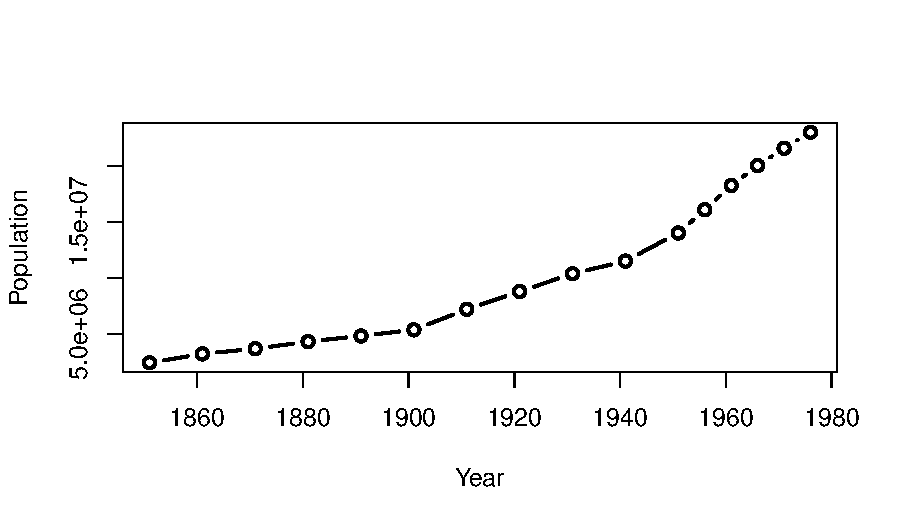
\includegraphics[width=\maxwidth]{FIGS/L05-plot-old-Canada-census-data-1} 
\end{knitrout}
\end{frame}


\begin{frame}[fragile]
But wait, this is only to 1976..! 
\vfill
Looking around, we find another table here
\vfill
There's a download csv link in there, let us see where this leads us
\begin{knitrout}
\definecolor{shadecolor}{rgb}{0.969, 0.969, 0.969}\color{fgcolor}\begin{kframe}
\begin{alltt}
\hldef{data_new} \hlkwb{=} \hlkwd{read.csv}\hldef{(}\hlsng{"https://www12.statcan.gc.ca/census-recensement/2011/dp-pd/vc-rv/download-telecharger/download-telecharger.cfm?Lang=eng&CTLG=98-315-XWE2011001&FMT=csv"}\hldef{)}
\end{alltt}
\end{kframe}
\end{knitrout}
The table is 720KB, so surely there must be more to this than just the population
\vfill
To get a sense of that, we dump a few random rows
\end{frame}

\begin{frame}[fragile]
\begin{knitrout}
\definecolor{shadecolor}{rgb}{0.969, 0.969, 0.969}\color{fgcolor}\begin{kframe}
\begin{alltt}
\hldef{data_new[}\hlkwd{sort}\hldef{(}\hlkwd{unique}\hldef{(}\hlkwd{c}\hldef{(}\hlnum{1}\hldef{,}\hlkwd{sample}\hldef{(}\hlkwd{nrow}\hldef{(data_new),} \hlnum{4}\hldef{)))), ]}
\end{alltt}
\begin{verbatim}
##                 GEOGRAPHY.NAME
## 1                       Canada
## 444  Newfoundland and Labrador
## 2628                 Qu\xe9bec
## 3814                  Kingston
## 6603                  Manitoba
##                                            CHARACTERISTIC YEAR.S.    TOTAL
## 1                               Population (in thousands)    1956 16081.00
## 444           Population by single years of age: 67 years    2011  5710.00
## 2628 Population change by broad age groups: 0 to 14 years    2001    -6.50
## 3814           % of the population aged 65 years and over    2011    16.30
## 6603                            % of lone-parent families    2001    16.23
##      FLAG_TOTAL
## 1              
## 444            
## 2628           
## 3814           
## 6603
\end{verbatim}
\end{kframe}
\end{knitrout}
\end{frame}


\begin{frame}{Flat tables}
This is a \defword{flat table}: each row contains a piece of information, the columns describe what this piece of information is about
\vfill
This has \emph{way more} information than we need: we just want the population of Canada and here we get 9960 rows over 213 characteristics
\vfill
Also, population is expressed in thousands, so once we selected what we want, we need to multiply by 1,000
\end{frame}

\begin{frame}[fragile]{Selecting rows}
We want the rows where the geography is ``Canada'' and the characteristic is ``Population (in thousands)''
\vfill
Find indices of rows that satisfy the first criterion and those that satisfy the second; intersecting these two sets of indices, we have selected the rows we want
\vfill
\begin{knitrout}
\definecolor{shadecolor}{rgb}{0.969, 0.969, 0.969}\color{fgcolor}\begin{kframe}
\begin{alltt}
\hldef{idx_CAN} \hlkwb{=} \hlkwd{which}\hldef{(data_new}\hlopt{$}\hldef{GEOGRAPHY.NAME} \hlopt{==} \hlsng{"Canada"}\hldef{)}
\hldef{idx_char} \hlkwb{=} \hlkwd{which}\hldef{(data_new}\hlopt{$}\hldef{CHARACTERISTIC} \hlopt{==} \hlsng{"Population (in thousands)"}\hldef{)}
\hldef{idx_keep} \hlkwb{=} \hlkwd{intersect}\hldef{(idx_CAN, idx_char)}
\end{alltt}
\end{kframe}
\end{knitrout}
\end{frame}


\begin{frame}[fragile]
Let us keep only these rows
\begin{knitrout}
\definecolor{shadecolor}{rgb}{0.969, 0.969, 0.969}\color{fgcolor}\begin{kframe}
\begin{alltt}
\hldef{data_new} \hlkwb{=} \hldef{data_new[idx_keep,]}
\hlkwd{head}\hldef{(data_new,} \hlkwc{n} \hldef{=} \hlnum{8}\hldef{)}
\end{alltt}
\begin{verbatim}
##   GEOGRAPHY.NAME            CHARACTERISTIC YEAR.S. TOTAL FLAG_TOTAL
## 1         Canada Population (in thousands)    1956 16081           
## 2         Canada Population (in thousands)    1961 18238           
## 3         Canada Population (in thousands)    1966 20015           
## 4         Canada Population (in thousands)    1971 21568           
## 5         Canada Population (in thousands)    1976 22993           
## 6         Canada Population (in thousands)    1981 24343           
## 7         Canada Population (in thousands)    1986 25309           
## 8         Canada Population (in thousands)    1991 27297
\end{verbatim}
\end{kframe}
\end{knitrout}
\end{frame}


\begin{frame}
We want to concatenate this data frame with the one from earlier
\vfill
To do this, we need the two data frames to have the same number of columns, same column names and same entry types (notice that \code{YEAR.S.} in \code{data\_new} is a column of characters)
\end{frame}

\begin{frame}\frametitle{What remains to be done}
\begin{itemize}
\item Rename the columns in the pruned old data (data\_pruned) to \code{year} and \code{population}. Personally, I prefer lowercase column names.. and \code{population} is more informative than \code{Canada}
\vfill
\item Keep only the relevant columns in \code{data\_new}, rename them accordingly and multiply population by 1,000 there
\vfill
\item Transform year in \code{data\_new} to numbers
\vfill
\item We already have data up to and including 1976 in \code{data\_old}, so get rid of that in \code{data\_new}
\vfill
\item Append the rows of \code{data\_new} to those of \code{data\_pruned}
\end{itemize}
\end{frame}


\begin{frame}[fragile]
\begin{knitrout}
\definecolor{shadecolor}{rgb}{0.969, 0.969, 0.969}\color{fgcolor}\begin{kframe}
\begin{alltt}
\hlkwd{colnames}\hldef{(data_old)} \hlkwb{=} \hlkwd{c}\hldef{(}\hlsng{"year"}\hldef{,} \hlsng{"population"}\hldef{)}
\hldef{data_new} \hlkwb{=} \hldef{data_new[,}\hlkwd{c}\hldef{(}\hlsng{"YEAR.S."}\hldef{,}\hlsng{"TOTAL"}\hldef{)]}
\hlkwd{colnames}\hldef{(data_new)} \hlkwb{=} \hlkwd{c}\hldef{(}\hlsng{"year"}\hldef{,} \hlsng{"population"}\hldef{)}
\hldef{data_new}\hlopt{$}\hldef{year} \hlkwb{=} \hlkwd{as.numeric}\hldef{(data_new}\hlopt{$}\hldef{year)}
\hldef{data_new} \hlkwb{=} \hldef{data_new[}\hlkwd{which}\hldef{(data_new}\hlopt{$}\hldef{year}\hlopt{>}\hlnum{1976}\hldef{),]}
\hldef{data_new}\hlopt{$}\hldef{population} \hlkwb{=} \hldef{data_new}\hlopt{$}\hldef{population}\hlopt{*}\hlnum{1000}

\hldef{data} \hlkwb{=} \hlkwd{rbind}\hldef{(data_old,data_new)}
\end{alltt}
\end{kframe}
\end{knitrout}
\end{frame}


\begin{frame}[fragile]
\begin{knitrout}
\definecolor{shadecolor}{rgb}{0.969, 0.969, 0.969}\color{fgcolor}\begin{kframe}
\begin{alltt}
\hlkwd{plot}\hldef{(data}\hlopt{$}\hldef{year, data}\hlopt{$}\hldef{population,}
    \hlkwc{type} \hldef{=} \hlsng{"b"}\hldef{,} \hlkwc{lwd} \hldef{=} \hlnum{2}\hldef{,}
    \hlkwc{xlab} \hldef{=} \hlsng{"Year"}\hldef{,} \hlkwc{ylab} \hldef{=} \hlsng{"Population"}\hldef{)}
\end{alltt}
\end{kframe}
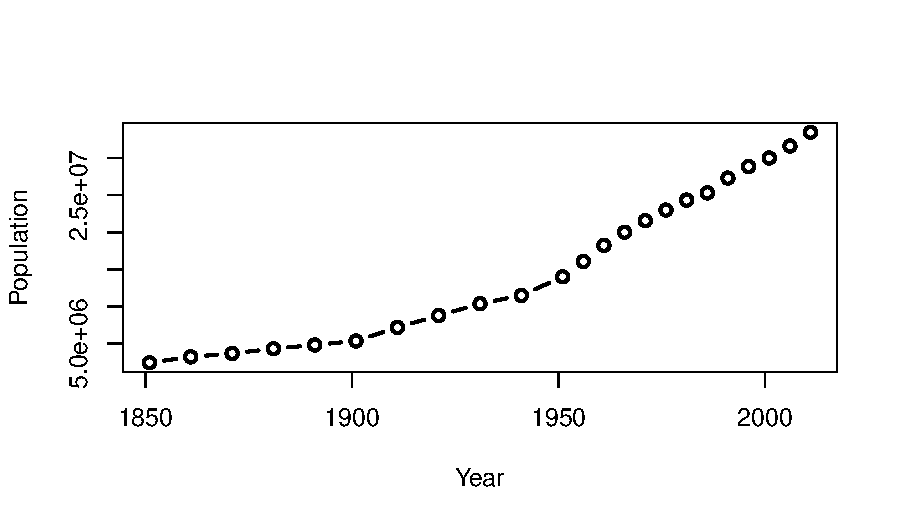
\includegraphics[width=\maxwidth]{FIGS/L05-plot-whole-Canada-census-data-1} 
\end{knitrout}
\end{frame}

\begin{frame}[fragile]\frametitle{Save the processed data}
In case we need the data elsewhere, we save the data to a \code{csv} file
\vfill
\begin{knitrout}
\definecolor{shadecolor}{rgb}{0.969, 0.969, 0.969}\color{fgcolor}\begin{kframe}
\begin{alltt}
\hlkwd{write.csv}\hldef{(data,} \hlkwc{file} \hldef{=} \hlsng{"../CODE/Canada_census.csv"}\hldef{)}
\end{alltt}
\end{kframe}
\end{knitrout}
\vfill
Using \code{readr} saves the data without row numbers (by default), so we can do this instead
\vfill
\begin{knitrout}
\definecolor{shadecolor}{rgb}{0.969, 0.969, 0.969}\color{fgcolor}\begin{kframe}
\begin{alltt}
\hldef{readr}\hlopt{::}\hlkwd{write_csv}\hldef{(data,} \hlkwc{file} \hldef{=} \hlsng{"../CODE/Canada_census.csv"}\hldef{)}
\end{alltt}
\end{kframe}
\end{knitrout}
\end{frame}

%%%%%%%%%%%%%%%%%%%%%
%%%%%%%%%%%%%%%%%%%%%
\Ssection{Least squares problem -- Initial considerations}{FIGS-slides-admin/Gemini_Generated_Image_gc7vxngc7vxngc7v.jpeg}

\begin{frame}
We just collected the census data for Canada
\vfill
Suppose we want to predict the population of Canada in 20 years given the historical population growth seen in the previous plot. What can we do?
\vfill
If there were just two points, we could easily "drive" a line through these two points. However, we have much more than two points, so we will use \emph{fitting}, \emph{i.e.}, try to make a curve come as close to possible to the points
\vfill
We start with a line, giving rise to \defword{linear least squares}
\end{frame}

\begin{frame}[fragile]\frametitle{Least squares approximation -- A trivial case}
\begin{knitrout}
\definecolor{shadecolor}{rgb}{0.969, 0.969, 0.969}\color{fgcolor}
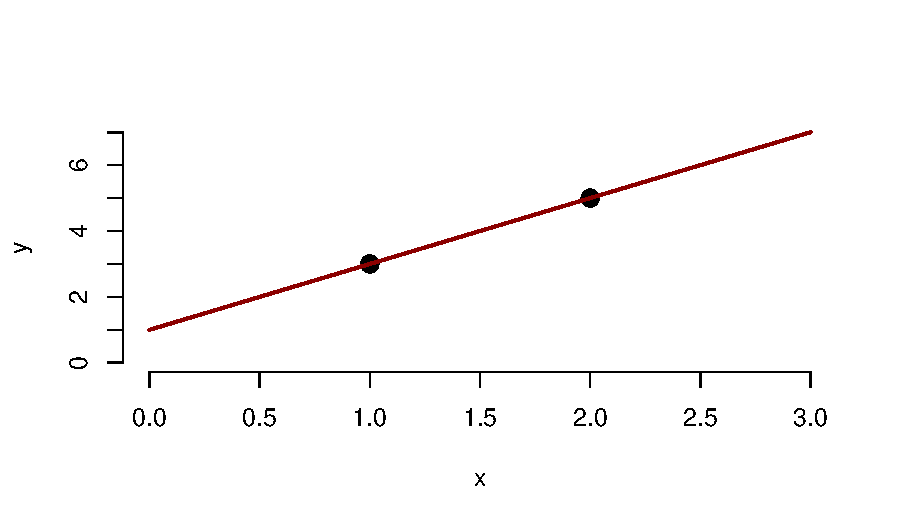
\includegraphics[width=\maxwidth]{FIGS/L05-plot-2-points-and-line-1} 
\end{knitrout}
\end{frame}

\begin{frame}
We want to find the equation of a line $y=a+bx$ that goes through these two points, i.e., we seek $a$ and $b$ such that
$$
\begin{aligned}
3 &= a+b \\
5 &= a+2b
\end{aligned}
$$
i.e., they satisfy $y=a+bx$ for $(x,y)=(1,3)$ and $(x,y)=(2,5)$
\end{frame}

\begin{frame}
This is a linear system with 2 equations and 2 unknowns $a$ and $b$
$$
\begin{pmatrix}
1 & 1 \\ 1 & 2
\end{pmatrix}
\begin{pmatrix}
a \\ b
\end{pmatrix}
=
\begin{pmatrix}
3 \\ 5
\end{pmatrix}
$$
\end{frame}

\begin{frame}[fragile]
We know from the ``famous'' linear algebra in a nutshell theorem that this system has a unique solution if the matrix
$$
M=
\begin{pmatrix}
1 & 1 \\ 1 & 2
\end{pmatrix}
$$
is invertible
\vfill
$\det(M)=1$, so we are good, we'll find $a$ and $b$ easily..
\end{frame}

\begin{frame}[fragile]
Now let's add another point
\begin{knitrout}
\definecolor{shadecolor}{rgb}{0.969, 0.969, 0.969}\color{fgcolor}\begin{kframe}
\begin{alltt}
\hldef{points} \hlkwb{=} \hlkwd{list}\hldef{()}
\hldef{points}\hlopt{$}\hldef{x} \hlkwb{=} \hlkwd{c}\hldef{(}\hlnum{1}\hldef{,}\hlnum{2}\hldef{,}\hlnum{3}\hldef{)}
\hldef{points}\hlopt{$}\hldef{y} \hlkwb{=} \hlkwd{c}\hldef{(}\hlnum{3}\hldef{,}\hlnum{5}\hldef{,}\hlnum{4}\hldef{)} \hlcom{# So the points are (1,3), (2,5) and (3,4)}
\hlkwd{plot}\hldef{(points}\hlopt{$}\hldef{x, points}\hlopt{$}\hldef{y,}
     \hlkwc{pch} \hldef{=} \hlnum{19}\hldef{,} \hlkwc{cex} \hldef{=} \hlnum{2}\hldef{,} \hlkwc{bty} \hldef{=} \hlsng{"n"}\hldef{,}
    \hlkwc{xlim} \hldef{=} \hlkwd{c}\hldef{(}\hlnum{0}\hldef{,} \hlnum{3.5}\hldef{),} \hlkwc{ylim} \hldef{=} \hlkwd{c}\hldef{(}\hlnum{0}\hldef{,}\hlnum{6}\hldef{),} \hlkwc{xlab} \hldef{=} \hlsng{"x"}\hldef{,} \hlkwc{ylab} \hldef{=} \hlsng{"y"}\hldef{)}
\end{alltt}
\end{kframe}
\end{knitrout}
These points are clearly not colinear, so there is not one line going through the 3
\end{frame}

\begin{frame}
We end up with an *overdetermined* system
$$
\begin{aligned}
3 &= a+b \\
5 &= a+2b \\
4 &= a+3b
\end{aligned}
$$
i.e.,
$$
\begin{pmatrix}
1 & 1 \\ 1 & 2 \\ 1 & 3
\end{pmatrix}
\begin{pmatrix}
a \\ b
\end{pmatrix}
=
\begin{pmatrix}
3 \\ 5 \\ 4
\end{pmatrix}
$$
\end{frame}

\begin{frame}[fragile]
We have verified visually that the points are not colinear, so this system has no solution.

(If you had to do it for good, you consider two vectors stemming from these 3 points and compute the angle between them or check that one is a multiple of the other).

So let us instead try to find the line that comes "closest" to the 3 points.

\begin{knitrout}
\definecolor{shadecolor}{rgb}{0.969, 0.969, 0.969}\color{fgcolor}\begin{kframe}
\begin{alltt}
\hldef{A} \hlkwb{=} \hlkwd{matrix}\hldef{(}\hlkwd{c}\hldef{(}\hlnum{1}\hldef{,}\hlnum{1}\hldef{,}\hlnum{1}\hldef{,}\hlnum{2}\hldef{),} \hlkwc{nr} \hldef{=} \hlnum{2}\hldef{,} \hlkwc{nc} \hldef{=} \hlnum{2}\hldef{,} \hlkwc{byrow} \hldef{=} \hlnum{TRUE}\hldef{)}
\hldef{rhs} \hlkwb{=} \hlkwd{matrix}\hldef{(}\hlkwd{c}\hldef{(}\hlnum{3}\hldef{,}\hlnum{5}\hldef{),} \hlkwc{nr} \hldef{=} \hlnum{2}\hldef{,} \hlkwc{nc} \hldef{=}\hlnum{1}\hldef{)}
\hldef{coefs} \hlkwb{=} \hlkwd{solve}\hldef{(A,rhs)} \hlcom{# To invert A, in R, you use solve(A), to solve Ax=b, you use solve(A,b)}
\hlkwd{plot}\hldef{(points}\hlopt{$}\hldef{x, points}\hlopt{$}\hldef{y,}
     \hlkwc{pch} \hldef{=} \hlnum{19}\hldef{,} \hlkwc{cex} \hldef{=} \hlnum{2}\hldef{,} \hlkwc{bty} \hldef{=} \hlsng{"n"}\hldef{,}
    \hlkwc{xlim} \hldef{=} \hlkwd{c}\hldef{(}\hlnum{0}\hldef{,} \hlnum{3.5}\hldef{),} \hlkwc{ylim} \hldef{=} \hlkwd{c}\hldef{(}\hlnum{0}\hldef{,}\hlnum{6}\hldef{),} \hlkwc{xlab} \hldef{=} \hlsng{"x"}\hldef{,} \hlkwc{ylab} \hldef{=} \hlsng{"y"}\hldef{)}
\hlkwd{abline}\hldef{(}\hlkwc{coef} \hldef{= coefs,} \hlkwc{lwd} \hldef{=} \hlnum{2}\hldef{)}
\end{alltt}
\end{kframe}
\end{knitrout}

Obviously, not sensational..
\end{frame}

\begin{frame}[fragile]
\begin{knitrout}
\definecolor{shadecolor}{rgb}{0.969, 0.969, 0.969}\color{fgcolor}\begin{kframe}
\begin{alltt}
\hlkwd{plot}\hldef{(points}\hlopt{$}\hldef{x, points}\hlopt{$}\hldef{y,}
     \hlkwc{pch} \hldef{=} \hlnum{19}\hldef{,} \hlkwc{cex} \hldef{=} \hlnum{2}\hldef{,} \hlkwc{bty} \hldef{=} \hlsng{"n"}\hldef{,}
    \hlkwc{xlim} \hldef{=} \hlkwd{c}\hldef{(}\hlnum{0}\hldef{,} \hlnum{3.5}\hldef{),} \hlkwc{ylim} \hldef{=} \hlkwd{c}\hldef{(}\hlnum{0}\hldef{,}\hlnum{6}\hldef{),} \hlkwc{xlab} \hldef{=} \hlsng{"x"}\hldef{,} \hlkwc{ylab} \hldef{=} \hlsng{"y"}\hldef{)}
\hlkwd{abline}\hldef{(}\hlkwc{coef} \hldef{= coefs,} \hlkwc{lwd} \hldef{=} \hlnum{2}\hldef{)}
\hlkwd{abline}\hldef{(}\hlkwc{a} \hldef{=} \hlnum{3}\hldef{,} \hlkwc{b} \hldef{=} \hlnum{0.5}\hldef{,} \hlkwc{lwd} \hldef{=} \hlnum{2}\hldef{,} \hlkwc{col} \hldef{=} \hlsng{"red"}\hldef{)}
\end{alltt}
\end{kframe}
\end{knitrout}

How do we find "how far away"?

- We could use projections onto the line (which we know minimises the distance)
- However, this will be a problem if we later decide that rather than a straight line, we want to use something more "funky" like a quadratic or an exponential
\end{frame}


\begin{frame}
So instead, we compare, for a given value $x$, the distance between the true value $y$ and the value of $y$ obtained using the curve (line, here) that we use to fit the data

Let $(x_i,y_i)$ be the data points, i.e., here, $(x_1,y_1)=(1,3)$, $(x_2,y_2)=(2,5)$ and $(x_3,y_3)=(3,4)$

Now suppose we use a line with equation $y=a+bx$ and that we pick a value for $a$ and $b$. Then at $x_1$,
$$
\tilde y_1 = a+bx_1 = a+b
$$
at $x_2$
$$
\tilde y_2 = a+bx_2 = a+2b
$$
and at $x_3$,
$$
\tilde y_3 = a+bx_3 = a+3b
$$
Consider $x_1$, for instance. The error we made by using the line with coefficients $(a,b)$ is $\overrightarrow{(x_1,y_1)(x_1,\tilde y_1)}$.
\end{frame}

\begin{frame}[fragile]
For future use, let us create a function for $y = a_0 + a_1x$.

\begin{knitrout}
\definecolor{shadecolor}{rgb}{0.969, 0.969, 0.969}\color{fgcolor}\begin{kframe}
\begin{alltt}
\hldef{my_line} \hlkwb{=} \hlkwa{function}\hldef{(}\hlkwc{x}\hldef{,} \hlkwc{a_0}\hldef{,} \hlkwc{a_1}\hldef{)\{}
    \hlkwd{return}\hldef{(a_0} \hlopt{+} \hldef{a_1}\hlopt{*}\hldef{x)}
\hldef{\}}
\end{alltt}
\end{kframe}
\end{knitrout}

Functions are super useful when programming

\begin{knitrout}
\definecolor{shadecolor}{rgb}{0.969, 0.969, 0.969}\color{fgcolor}\begin{kframe}
\begin{alltt}
\hlkwd{my_line}\hldef{(}\hlnum{1}\hldef{,}\hlnum{2}\hldef{,}\hlnum{3}\hldef{)}
\end{alltt}
\begin{verbatim}
## [1] 5
\end{verbatim}
\begin{alltt}
\hlkwd{my_line}\hldef{(}\hlkwc{a_0} \hldef{=} \hlnum{2}\hldef{,} \hlkwc{a_1} \hldef{=} \hlnum{3}\hldef{,} \hlkwc{x} \hldef{=} \hlnum{1}\hldef{)}
\end{alltt}
\begin{verbatim}
## [1] 5
\end{verbatim}
\begin{alltt}
\hlkwd{my_line}\hldef{(}\hlkwc{x} \hldef{=} \hlkwd{c}\hldef{(}\hlnum{1}\hldef{,}\hlnum{2}\hldef{,}\hlnum{3}\hldef{),} \hlkwc{a_0} \hldef{=} \hlnum{2}\hldef{,} \hlkwc{a_1} \hldef{=} \hlnum{3}\hldef{)}
\end{alltt}
\begin{verbatim}
## [1]  5  8 11
\end{verbatim}
\end{kframe}
\end{knitrout}
\end{frame}


\begin{frame}[fragile]
\begin{knitrout}
\definecolor{shadecolor}{rgb}{0.969, 0.969, 0.969}\color{fgcolor}\begin{kframe}
\begin{alltt}
\hldef{a} \hlkwb{=} \hlnum{3}
\hldef{b} \hlkwb{=} \hlnum{0.5} \hlcom{# The line has equation y=a+bx}
\hlkwd{plot}\hldef{(points}\hlopt{$}\hldef{x, points}\hlopt{$}\hldef{y,}
     \hlkwc{pch} \hldef{=} \hlnum{19}\hldef{,} \hlkwc{cex} \hldef{=} \hlnum{2}\hldef{,} \hlkwc{bty} \hldef{=} \hlsng{"n"}\hldef{,}
    \hlkwc{xlim} \hldef{=} \hlkwd{c}\hldef{(}\hlnum{0}\hldef{,} \hlnum{3.5}\hldef{),} \hlkwc{ylim} \hldef{=} \hlkwd{c}\hldef{(}\hlnum{0}\hldef{,}\hlnum{6}\hldef{),} \hlkwc{xlab} \hldef{=} \hlsng{"x"}\hldef{,} \hlkwc{ylab} \hldef{=} \hlsng{"y"}\hldef{)}
\hlkwd{abline}\hldef{(}\hlkwc{a} \hldef{= a,} \hlkwc{b} \hldef{= b,} \hlkwc{lwd} \hldef{=} \hlnum{2}\hldef{)}
\hlkwd{abline}\hldef{(}\hlkwc{v} \hldef{=} \hlkwd{c}\hldef{(}\hlnum{1}\hldef{,}\hlnum{2}\hldef{,}\hlnum{3}\hldef{))}  \hlcom{# If we used abline(h=c(0,1)), we would get horizontal lines at y=0 and y=1}
\hldef{p} \hlkwb{=} \hlkwd{my_line}\hldef{(}\hlkwd{c}\hldef{(}\hlnum{1}\hldef{,}\hlnum{2}\hldef{,}\hlnum{3}\hldef{), a, b)}
\hlkwd{points}\hldef{(}\hlkwd{c}\hldef{(}\hlnum{1}\hldef{,}\hlnum{2}\hldef{,}\hlnum{3}\hldef{), p,} \hlkwc{pch} \hldef{=} \hlnum{19}\hldef{,} \hlkwc{cex} \hldef{=} \hlnum{2}\hldef{,} \hlkwc{col} \hldef{=} \hlsng{"red"}\hldef{)}
\end{alltt}
\end{kframe}
\end{knitrout}
\end{frame}

\begin{frame}
Let us return to the error
$$
\overrightarrow{(x_1,y_1)(x_1,\tilde y_1)}
$$
We have
$$
\overrightarrow{(x_1,y_1)(x_1,\tilde y_1)}
= (x_1-x_1,y_1-\tilde y_1)
= (0, y_1-\tilde y_1)
$$
Let us call
$$
\varepsilon_1 = y_1-\tilde y_1
$$
We can compute $\varepsilon_2$ and $\varepsilon_3$ too. And we can then form the **error vector**
$$
\mathbf{e} = (\varepsilon_1,\varepsilon_2,\varepsilon_3)^T
$$
The norm of $\mathbf{e}$, $\|\mathbf{e}\|$, then tells us how much error we are making for the choice of $(a,b)$ we are using
\end{frame}


\begin{frame}
The norm of $\mathbf{e}$, $\|\mathbf{e}\|$, tells us how much error we are making for the choice of $(a,b)$ we are using

So our objective is to find $(a,b)$ such that $\|\mathbf{e}\|$ is minimal

We could use various norms, but the Euclidean norm has some very interesting properties, so we use
$$
\|\mathbf{e}\| = \sqrt{\varepsilon_1^2+\varepsilon_2^2+\varepsilon_3^2}
$$
\end{frame}


\begin{frame}\frametitle{The linear least squares problem}
Given a collection of data points $(x_1,y_1),\ldots,(x_n,y_n)$, find the coefficients $a,b$ of the line $y=a+bx$ such that
$$
\|\mathbf{e}\|=\sqrt{\varepsilon_1^2+\cdots+\varepsilon_n^2}
=\sqrt{(y_1-\tilde y_1)^2+\cdots+(y_n-\tilde y_n)^2}
$$
is minimal, where $\tilde y_i=a+bx_i$, for $i=1,\ldots,n$
\end{frame}


\begin{frame}[fragile]
Let us first hack a brute force solution! (For the example we have been using this far)

We have our three points in the list `points`, the function \code{my\_line} that computes the value $\tilde y$ given $x$ and $a,b$, so let us make a new function that, given $a,b$, computes $\mathbf{e}$

We'll also pass the points `points`

\begin{knitrout}
\definecolor{shadecolor}{rgb}{0.969, 0.969, 0.969}\color{fgcolor}\begin{kframe}
\begin{alltt}
\hldef{error} \hlkwb{=} \hlkwa{function}\hldef{(}\hlkwc{a_0}\hldef{,} \hlkwc{a_1}\hldef{,} \hlkwc{points}\hldef{) \{}
    \hldef{y_tilde} \hlkwb{=} \hlkwd{my_line}\hldef{(points}\hlopt{$}\hldef{x,} \hlkwc{a_0} \hldef{= a_0,} \hlkwc{a_1} \hldef{= a_1)}
    \hldef{e} \hlkwb{=} \hldef{points}\hlopt{$}\hldef{y} \hlopt{-} \hldef{y_tilde}
    \hlkwd{return}\hldef{(}\hlkwd{sqrt}\hldef{(}\hlkwd{sum}\hldef{(e}\hlopt{^}\hlnum{2}\hldef{)))}
\hldef{\}}
\hlkwd{error}\hldef{(}\hlkwc{a_0} \hldef{=} \hlnum{2}\hldef{,} \hlkwc{a_1} \hldef{=} \hlnum{3}\hldef{, points)}
\end{alltt}
\begin{verbatim}
## [1] 7.874008
\end{verbatim}
\begin{alltt}
\hlkwd{error}\hldef{(}\hlkwc{a_0} \hldef{=} \hlnum{3}\hldef{,} \hlkwc{a_1} \hldef{=} \hlnum{0.5}\hldef{, points)}
\end{alltt}
\begin{verbatim}
## [1] 1.224745
\end{verbatim}
\begin{alltt}
\hlkwd{error}\hldef{(}\hlkwc{a_0} \hldef{=} \hlnum{3.1}\hldef{,} \hlkwc{a_1} \hldef{=} \hlnum{0.48}\hldef{, points)}
\end{alltt}
\begin{verbatim}
## [1] 1.229471
\end{verbatim}
\end{kframe}
\end{knitrout}

We can't be doing this by hand..
\end{frame}


\begin{frame}\frametitle{Let's minimise using something cool -- \emph{genetic algorithms}}


\begin{itemize}
\item Genetic algorithms are a stochastic *optimisation* method. There are other types, e.g., gradient descent (deterministic)
\item The idea is to use a mechanism mimicking evolution's drive towards higher fitness
\item The function value is its fitness
\item We try different genes (here, different values of $a,b$) and evaluate their fitness.. keep the good ones
\item We mutate or crossover genes, throw in new ones, etc.
\item We keep doing this until we reach a stopping criterion
\item We then return the best gene we found
\end{itemize}
\end{frame}


\begin{frame}[fragile]
\begin{knitrout}
\definecolor{shadecolor}{rgb}{0.969, 0.969, 0.969}\color{fgcolor}\begin{kframe}
\begin{alltt}
\hlkwa{if} \hldef{(}\hlopt{!}\hlkwd{require}\hldef{(}\hlsng{"GA"}\hldef{,} \hlkwc{quietly} \hldef{=} \hlnum{TRUE}\hldef{)) \{}
  \hlkwd{install.packages}\hldef{(}\hlsng{"GA"}\hldef{)}
  \hlkwd{library}\hldef{(GA)}
\hldef{\}}
\hldef{GA} \hlkwb{=} \hlkwd{ga}\hldef{(}\hlkwc{type} \hldef{=} \hlsng{"real-valued"}\hldef{,}
        \hlkwc{fitness} \hldef{=} \hlkwa{function}\hldef{(}\hlkwc{x}\hldef{)} \hlopt{-}\hlkwd{error}\hldef{(}\hlkwc{a_0} \hldef{= x[}\hlnum{1}\hldef{],} \hlkwc{a_1} \hldef{= x[}\hlnum{2}\hldef{], points),}
        \hlkwc{suggestions} \hldef{=} \hlkwd{c}\hldef{(}\hlkwc{a_0} \hldef{=} \hlnum{2}\hldef{,} \hlkwc{a_1} \hldef{=} \hlnum{3}\hldef{),}
        \hlkwc{lower} \hldef{=} \hlkwd{c}\hldef{(}\hlopt{-}\hlnum{10}\hldef{,} \hlopt{-}\hlnum{10}\hldef{),} \hlkwc{upper} \hldef{=} \hlkwd{c}\hldef{(}\hlnum{10}\hldef{,} \hlnum{10}\hldef{),}
        \hlkwc{popSize} \hldef{=} \hlnum{200}\hldef{,} \hlkwc{maxiter} \hldef{=} \hlnum{150}\hldef{)}
\hlcom{# plot(GA)}
\hldef{GA}
\end{alltt}
\begin{verbatim}
## An object of class "ga"
## 
## Call:
## ga(type = "real-valued", fitness = function(x) -error(a_0 = x[1],     a_1 = x[2], points), lower = c(-10, -10), upper = c(10, 10),     popSize = 200, maxiter = 150, suggestions = c(a_0 = 2, a_1 = 3))
## 
## Available slots:
##  [1] "call"         "type"         "lower"        "upper"        "nBits"       
##  [6] "names"        "popSize"      "iter"         "run"          "maxiter"     
## [11] "suggestions"  "population"   "elitism"      "pcrossover"   "pmutation"   
## [16] "optim"        "fitness"      "summary"      "bestSol"      "fitnessValue"
## [21] "solution"
\end{verbatim}
\begin{alltt}
\hldef{GA}\hlopt{@}\hlkwc{solution}
\end{alltt}
\begin{verbatim}
##            x1        x2
## [1,] 3.000767 0.4996946
\end{verbatim}
\begin{alltt}
\hlopt{-}\hldef{GA}\hlopt{@}\hlkwc{fitnessValue}
\end{alltt}
\begin{verbatim}
## [1] 1.224745
\end{verbatim}
\end{kframe}
\end{knitrout}
\end{frame}

\begin{frame}
\begin{itemize}
\item Here, however, we do not have to go brute force: we can reason using mathematics
\item We now take a little detour on the math side of things, we will come back to code in a while..
\end{itemize}
\end{frame}







% Save counters for next file

% Save theorem count for next file
\end{document}
